% @file:	tmp.tex
% @author:	Jacob Xie
% @date:	2023/04/10 22:50:05 Monday
% @brief:

\documentclass[../studies-ml.tex]{subfiles}

\begin{document}

\subsection*{ResNet 与 CNN}

\begin{equation*}
  \begin{aligned}
     & x_0 = \text{input image}                                              \\
     & x_n = F(x_{n-1}, {W_i}) + x_{n-1} \qquad \text{for} ; n = 1,2,\dots,N \\
     & \hat{y} = \text{softmax}(x_N)
  \end{aligned}
\end{equation*}

\begin{itemize}
  \item $x_0$: 输入的图像;
  \item $x_n$: 第 $n$ 层残差块的特征映射;
  \item $F$: 供神经网络所学习的残差函数;
  \item $W_i$: 供神经网络所学习的参数;
  \item $N$: 神经网络中残差块的数量;
  \item $\hat{y}$: 在最后一层残差块上所应用的 \textit{softmax} 函数,而得出的输出。
\end{itemize}

\begin{figure}[h]
  \centering
  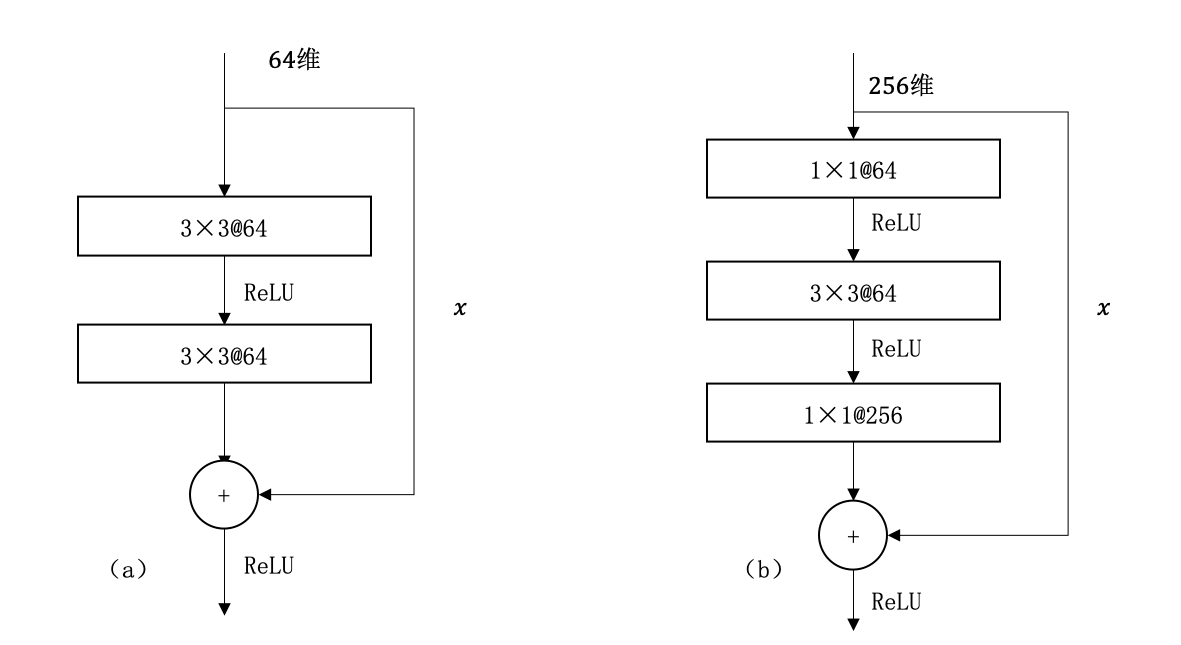
\includegraphics[width=0.6\textwidth]{\subfix{../images/ResNet-residual-block.png}}\par
  ResNet 残差块
\end{figure}

\begin{figure}[h]
  \centering
  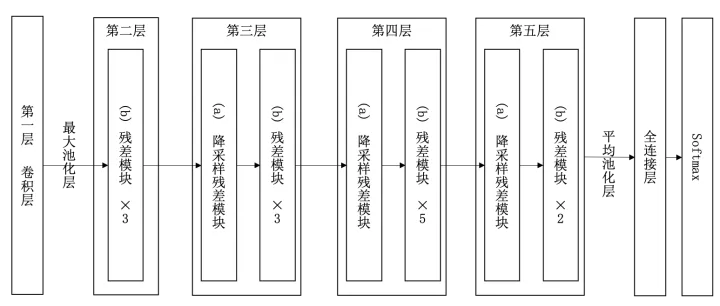
\includegraphics[width=0.6\textwidth]{\subfix{../images/ResNet-model-framework.png}}\par
  ResNet 模型框架
\end{figure}

Difference between a ResNet and a traditional neural network: the use of the residual function $F$,
which allows the network to learn residual mappings that add to the input of each residual block.
This allows for deeper networks to be trained without suffering from the vanishing gradient problem.

% TODO

\end{document}
